\documentclass{article}

\usepackage[italian]{babel}  % traduzioni + sillabazione

\usepackage{amsmath}
\usepackage{graphicx}
\usepackage{tikz}
\usetikzlibrary{shapes.geometric}
\usepackage[margin=1in]{geometry}

\begin{document}

\graphicspath{{./images}}

\tableofcontents

\section{Panoramica introduttiva}
Lo scopo del programma è quello di identificare dei percorsi minimi all'interno di una griglia esagonale.\\
Questa griglia mima possibili percorsi, via terra o aria, di mezzi che devono trovare il modo più efficiente per spostarsi da un punto A ad un punto B.\\
Le rotte possono essere modificate, editandone il costo, eliminate o aggiunte.\\\\
Infine, l'input al programma verrà pompato tramite \texttt{stdin}.\\
Si può simulare questo pompaggio tramite un file, con il comando:
\begin{center}
    \texttt{./program < input.txt}
\end{center}
Per salvare anche l'output:
\begin{center}
    \begin{center}
    \texttt{./program < input.txt > output.txt}
\end{center}
\end{center}

\section{Struttura costitutiva}
\subsection{Costruzione griglia}
La griglia è esagonale di forma rettangolare, di dimensione fissata all'inizio del programma. Ogni esagono è identificato dalle coordinate
\[\text{(column, row)}\]
Un esempio di griglia è la seguente:

\begin{center}
\begin{tikzpicture}[scale=0.9]
\tikzstyle{hex} = [draw, thick, regular polygon, regular polygon sides=6, minimum size=1.2cm, inner sep=0, rotate=30]

% Dimensioni
\def\ncols{5}
\def\nrows{4}

% Disegna esagoni
\foreach \row in {0,...,3} {
  \pgfmathtruncatemacro{\revrow}{3 - \row}
  \foreach \col in {0,...,4} {
    \pgfmathsetmacro\x{sqrt(3)*\col + mod(\row,2)*sqrt(3)/2}
    \pgfmathsetmacro\y{1.5*\row}
    \node[hex] at (\x,\y) {};
  }
}

% Etichette colonne
\foreach \c in {0,...,4} {
  \pgfmathsetmacro\x{sqrt(3)*\c}
  \node at (\x,-1) {\textbf{\c}};
}

% Etichette righe
\foreach \val/\y in {3/4.5, 2/3.0, 1/1.5, 0/0.0} {
  \node at (-1,\y) {\textbf{\val}};
}

\end{tikzpicture}
\end{center}

Si nota però che con questo sistema di coordinate, chiamato \textit{offset odd-r}:
\begin{itemize}
    \item \textit{Righe pari}: risultano ben allineate a sinistra
    \item \textit{Righe dispari}: risultano "spostate" di mezzo esagono a destra
\end{itemize}
Non permette le basilari operazioni vettoriali quali somma, sottrazione, moltiplicazioni per uno scalare \dots\\

È utile, per calcolare le distanze, passare da coordinate esagonali a \textbf{coordinate assiali}. Queste si compongono di:
\begin{itemize}
    \item \textbf{Row}: è la stessa delle coordinate esagonali
    \begin{center}
        \texttt{r = row}
    \end{center}
    \item \textbf{Oblique-Column}: rappresenta la posizione lungo una direzione obliqua che attraversa la griglia da nord-ovest a sud-est
    \begin{center}
        \texttt{q = column - (row >> 1)}
    \end{center}
    \begin{center}
        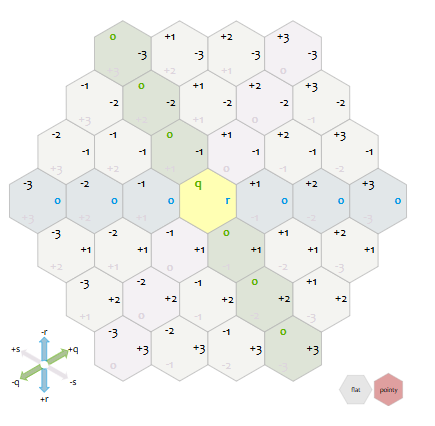
\includegraphics[scale=0.7]{axial}
    \end{center}
\end{itemize}

\subsection{Percorsi}
Ci sono due tipi di percorsi possibili:
\begin{itemize}
    \item \textbf{Percorso via terra}: collega automaticamente un esagono con i vicini
    \begin{itemize}
        \item \textbf{Esagono non abbandonabile}: ha costo 0 ed è un esagono da cui non si può partire via terra. Si può però \textit{visitare}.
        \item \textbf{Esagono abbandonabile}: ha un costo compreso tra 1-100
    \end{itemize}
    \item \textbf{Percorso via aria}: collega un esagono con al più 5 altri esagoni, in qualsiasi posizione essi siano
\end{itemize}
Ogni percorso è un numero naturale (non negativo).

\vspace{2em}

\begin{center}
\begin{tikzpicture}[scale=0.9]
\tikzstyle{hex} = [draw, thick, regular polygon, regular polygon sides=6, minimum size=1.2cm, inner sep=0, rotate=30]

% Dimensioni
\def\ncols{5}
\def\nrows{4}

% Disegna esagoni
\foreach \row in {0,...,3} {
  \foreach \col in {0,...,4} {

    % Coordinate geometriche
    \pgfmathsetmacro{\x}{sqrt(3)*\col + mod(\row,2)*sqrt(3)/2}
    \pgfmathsetmacro{\y}{1.5*\row}

    % 1) centro verde
    \pgfmathtruncatemacro{\isGreen}{(\row==1 && \col==2)}

    % 2) esagoni rossi
    \pgfmathtruncatemacro{\isRed}{
        (\row==2 && \col==1) ||
        (\row==2 && \col==3)
    }

    % 3) percorso non disponibile
    \pgfmathtruncatemacro{\isGrey}{
        (\row==1 && \col==1) ||
        (\row==0 && \col==2) ||
        (\row==0 && \col==3) ||
        (\row==1 && \col==3) ||
        (\row==2 && \col==2)
    }

    % nome del nodo → h-r-c
    \edef\nodename{h-\row-\col}

    % Disegna
    \ifnum\isGreen=1
      \node[hex, fill=green!40] (\nodename) at (\x,\y){};
      \node at (\x,\y) {\bfseries 0};
    \else\ifnum\isRed=1
        \node[hex, fill=red!40] (\nodename) at (\x,\y){};
    \else\ifnum\isGrey=1
        \node[hex, fill=black!40] (\nodename) at (\x,\y){};
    \else
      \node[hex] at (\x,\y) {};
    \fi\fi\fi
  }
}

% --- Frecce con costi (dal verde h-1-2) ------------------------------
% verso i 2 rossi --> costo 1
\foreach \target in {h-2-1,h-2-3} {
   \draw[->,thick] (h-1-2) -- (\target)
        node[midway,above,sloped]{\small 1};
}

% Etichette colonne
\foreach \c in {0,...,4} {
  \pgfmathsetmacro\x{sqrt(3)*\c}
  \node at (\x,-1) {\textbf{\c}};
}

% Etichette righe
\foreach \val/\y in {3/4.5, 2/3.0, 1/1.5, 0/0.0} {
  \node at (-1,\y) {\textbf{\val}};

}

\end{tikzpicture}
\end{center}
\begin{center}
    Esagono (1,2) non può essere lasciato via terra. Può però essere lasciato per via aerea
\end{center}

\vspace{1em}

\begin{center}
\begin{tikzpicture}[scale=0.9]
\tikzstyle{hex} = [draw, thick, regular polygon, regular polygon sides=6, minimum size=1.2cm, inner sep=0, rotate=30]

% Dimensioni
\def\ncols{5}
\def\nrows{4}

% Disegna esagoni
\foreach \row in {0,...,3} {
  \foreach \col in {0,...,4} {

    % Coordinate geometriche
    \pgfmathsetmacro{\x}{sqrt(3)*\col + mod(\row,2)*sqrt(3)/2}
    \pgfmathsetmacro{\y}{1.5*\row}

    % 1) centro verde
    \pgfmathtruncatemacro{\isGreen}{(\row==1 && \col==2)}

    % 2) esagoni rossi
    \pgfmathtruncatemacro{\isRed}{
        (\row==0 && \col==2) ||
        (\row==0 && \col==3) ||
        (\row==1 && \col==3) ||
        (\row==2 && \col==1) ||
        (\row==2 && \col==2) ||
        (\row==2 && \col==3) ||
        (\row==1 && \col==1)
    }

    % nome del nodo → h-r-c
    \edef\nodename{h-\row-\col}

    % Disegna
    \ifnum\isGreen=1
      \node[hex, fill=green!40] (\nodename) at (\x,\y){};
      \node at (\x,\y) {\bfseries 5};
    \else\ifnum\isRed=1
        \node[hex, fill=red!40] (\nodename) at (\x,\y){};
    \else
      \node[hex] at (\x,\y) {};
    \fi\fi
  }
}

% --- Frecce con costi (dal verde h-1-2) ------------------------------
% verso i 2 rossi --> costo 1
\foreach \target in {h-2-1,h-2-3} {
   \draw[->,thick] (h-1-2) -- (\target)
        node[midway,above,sloped]{\small 1};
}

% Etichette colonne
\foreach \c in {0,...,4} {
  \pgfmathsetmacro\x{sqrt(3)*\c}
  \node at (\x,-1) {\textbf{\c}};
}

% Etichette righe
\foreach \val/\y in {3/4.5, 2/3.0, 1/1.5, 0/0.0} {
  \node at (-1,\y) {\textbf{\val}};
}

\end{tikzpicture}
\end{center}
\begin{center}
    Costo via terra: 5\\
    Costo via aerea: 1
\end{center}

\section{Operazioni eseguibili}

\begin{itemize}
    \item \texttt{init $\langle$ columns $\rangle$ $\langle$ rows $\rangle$}\\\\
    Inizializza o reinizializza una nuova griglia di dimensione:
    \[\text{rows} \;\times\; \text{columns}\]
    Stampando poi il messaggio: \texttt{OK}.

    I parametri settati sono:
    \begin{itemize}
        \item Costo esagoni: 1
        \item Rotte aeree: nessuna
    \end{itemize}

    \item \texttt{change\_cost $\langle$ column $\rangle$ $\langle$ row $\rangle$  $\langle$ param $\rangle$ $\langle$ radius $\rangle$}\\\\
    Dove:
    \begin{itemize}
        \item \texttt{param}: nuovo parametro di costo, compreso tra [-10, 10]
        \item \texttt{radius}: raggio entro cui applicare il cambiamento
    \end{itemize}
    In particolare il raggio modifica ogni esagono a distanza:
    \[\text{d}\;<\;\text{radius}\]
    La modifica dei costi viene applicata al costo dell'\textbf{esagono} e di ogni \textbf{rotta} uscente secondo la formula:
    \[\text{weight}_{(x_e,y_e)}=\text{weight}_{(x_e,y_e)}+\lfloor \langle \text{\texttt{param}} \rangle\;\times\;max(0, \frac{\langle \text{\texttt{radius}} \rangle - dist(x_e, y_e, \langle x \rangle, \langle y \rangle)}{\langle \text{\texttt{radius}} \rangle}) \rfloor \]
    
    Stampando poi:
    \begin{itemize}
        \item \texttt{OK}: se esagono valido
        \item \texttt{KO}: se l'esagono non è valido o $\langle$ radius $\rangle$=0
    \end{itemize}
    \(dist(x_e, y_e, \langle x \rangle, \langle y \rangle)\) è il numero minimo di esagoni da \textit{visitare} per arrivare a \((x_e,y_e)\) ingorando i vari impedimenti (rotte, costi, non abbandonabilità), destinazione inclusa.

    \item \texttt{toggle\_air\_route $\langle$ x1 $\rangle$ $\langle$ y1 $\rangle$ $\langle$ x2 $\rangle$ $\langle$ y2 $\rangle$}\\\\
    Abbiamo 2 casi:
    \begin{itemize}
        \item Rotta già presente: viene rimossa
        \item Rotta non presente: viene aggiunta una rotta tra i due esagoni, dove il nuovo costo è la media per difetto di \textit{tutte le connessioni uscenti dall'esagono 1 e del suo costo di uscita}. 
    \end{itemize}

    Stampando poi:
    \begin{itemize}
        \item \texttt{OK}: se esagoni validi
        \item \texttt{KO}: se uno dei due esagoni non è valido o se l'esagono 1 disponde già di 5 rotte
    \end{itemize}

    \item \texttt{travel\_cost $\langle$ x1 $\rangle$ $\langle$ y1 $\rangle$ $\langle$ x2 $\rangle$ $\langle$ y2 $\rangle$}\\\\
    Calcola il costo minimo per raggiungere l'esagono 2 a partire dall'esagono 1, ignorando il costo dell'esagono 2.\\\\
    Stampando poi:
    \begin{itemize}
        \item \texttt{weight}: il costo totale, differenziando via aria o via terra
        \item \texttt{0}: se 1 e 2 coincidono, ovvero la destinazione coincide con la partenza
        \item \texttt{-1}: se se uno dei due esagoni non è valido o se non sono collegati in alcun modo
    \end{itemize}
\end{itemize}

\subsection{Spunto di ottimizzazione}
\begin{itemize}
    \item \textbf{Comandi poco usati}: \texttt{change\_cost} e \texttt{toggle\_air\_route}
    \item \textbf{Comandi altamente usati}: \texttt{travel\_cost}\\
    Inoltre questo si concentra molto spesso su stesse zone della mappa: sorgente e destinazione sono spesso concentrate in una singola zona. Altre zone verranno completamente ignorate
\end{itemize}

\end{document}